\chapter{MatSE580 Guest Lecture 1 - Quick Guide to Manipulating Materials With \texttt{pymatgen}, Setting up \texttt{MongoDB}, and Getting Started with \texttt{pySIPFENN}} 
\label{chap:pysipfenntutorial1} 

\hypertarget{introduction}{%
\section{Introduction}\label{pysipfenntutorial:introduction}}

In this guest lecture, we will cover: 

\begin{enumerate}
    \item \protect\hyperlink{Manipulating-and-analyzing-materials}{Manipulating and analyzing materials} - using \href{https://github.com/materialsproject/pymatgen}{pymatgen}

    \item \protect\hyperlink{Setting-up-MongoDB}{Setting up a small NoSQL database on the cloud to synchronize decentralized processing} - using \href{https://www.mongodb.com/atlas}{MongoDB Atlas} Free Tier 

    \item \protect\hyperlink{pymongo}{Interacting with the database} - using \href{https://github.com/mongodb/mongo-python-driver}{pymongo} library

    \item \protect\hyperlink{pysipfenn-install}{Installing machine learning (ML) tools} to predict stability of materials - using \href{https://pysipfenn.readthedocs.io/en/stable/}{pySIPFENN}
\end{enumerate}

Before you begin, you will need to set up a few essential development
tools.

While not required, it is recommended first to set up a virtual
environment using venv or Conda. This ensures that one of the required
versions of Python (3.9+) is used and there are no dependency conflicts.
It often comes preinstalled, like in GitHub Codespaces and some Linux
distributions. You can quickly check that by running.

\begin{minted}[xleftmargin=3\parindent, fontsize=\small, bgcolor=subtlegray]{output}
conda --version
\end{minted}

And if it is not installed, you can follow the
(\href{https://docs.conda.io/en/latest/miniconda.html}{miniconda
instructions} ) for a quick clean setup.

Once you have Conda installed on your system, you can create a new
environment with:

\begin{minted}[xleftmargin=3\parindent, fontsize=\small, bgcolor=subtlegray]{output}
conda create -n 580demo python=3.10 jupyter numpy scipy
conda init
\end{minted}

Restart your terminal, and activate the environment with:

\begin{minted}[xleftmargin=3\parindent, fontsize=\small, bgcolor=subtlegray]{output}
conda activate 580demo
\end{minted}

At this point, you should be able to run
\texttt{jupyter notebook} and open this notebook in
your browser with it or select the kernel
\texttt{580demo} in VS Code (top-right corner) or other
IDEs.

First, we will import some libraries that ship with Python so that we
don't need to worry about getting them, and are used in this notebook:

\begin{minted}[xleftmargin=3\parindent, linenos=true, fontsize=\small]{python}
from pprint import pprint            # pretty printing
from collections import defaultdict  # convenience in the example
import os                            # file handling
from datetime import datetime        # time handling
from zoneinfo import ZoneInfo        # time handling
\end{minted}

Now, we need to use \texttt{pip} package manager to
install the rest of the libraries we will use. If you are using Conda,
you could also use \texttt{conda install} instead, but
it is more elaborate for non-Anaconda-default packages.

We start with \texttt{pymatgen}, used in the next part
of this notebook. To install it, simply remove the
\texttt{\#} in the following line and run it, or open a
terminal and run \texttt{pip install pymatgen}.

\begin{minted}[xleftmargin=3\parindent, linenos=true, fontsize=\small]{python}
!pip install pymatgen
\end{minted}

And then install \texttt{pymongo} used in the 2nd part:

\begin{minted}[xleftmargin=3\parindent, linenos=true, fontsize=\small]{python}
!pip install pymongo
\end{minted}

Now, you should be ready to go!

\hypertarget{manipulating-and-analyzing-materials}{%
\section{Manipulating and analyzing
materials}\label{pysipfenntutorial:manipulating-and-analyzing-materials}}

To start working with atomic structures, often referred to as atomic
configurations or simply materials, we must be able to represent and
manipulate them. One of the most powerful and mature tools to do so is
\href{https://github.com/materialsproject/pymatgen}{pymatgen}, which we
just installed. The critical component of pymatgen is its library of
representations of fundamental materials objects, such as
\texttt{Structure} and
\texttt{Molecule}, contained in the
\texttt{pymatgen.core} module. Let's import it and
create a simple cubic structure of Al just as we did in the DFTTK
tutorial last week:

\hypertarget{basics}{%
\subsection{Basics}\label{pysipfenntutorial:basics}}

\begin{minted}[xleftmargin=3\parindent, linenos=true, fontsize=\small]{python}
from pymatgen.core import Structure

s = Structure(
        lattice=[[4.0384, 0, 0], [0, 4.0384, 0], [0, 0, 4.0384]],
        species=['Al', 'Al', 'Al', 'Al'],
        coords=[[0.0, 0.0, 0.0], [0, 0.5, 0.5], [0.5, 0.0, 0.5], [0.5, 0.5, 0.0]]
    )
\end{minted}

Now, \texttt{s} holds our initialized structure, and we
can apply print on it to see what it looks like:

\begin{minted}[xleftmargin=3\parindent, linenos=true, fontsize=\small]{python}
print(s)
\end{minted}

\begin{minted}[xleftmargin=3\parindent, fontsize=\small, bgcolor=subtlegray]{output}
Full Formula (Al4)
Reduced Formula: Al
abc   :   4.038400   4.038400   4.038400
angles:  90.000000  90.000000  90.000000
pbc   :       True       True       True
Sites (4)
  #  SP      a    b    c
---  ----  ---  ---  ---
  0  Al    0    0    0
  1  Al    0    0.5  0.5
  2  Al    0.5  0    0.5
  3  Al    0.5  0.5  0
\end{minted}

\textbf{Initialized} is a critical word here because the
\texttt{Structure} object is not just a collection of
``numbers''. It holds a lot of information we can access using the
\texttt{Structure} object's attributes and methods. For
example, the density of the material is immediately available:

\begin{minted}[xleftmargin=3\parindent, linenos=true, fontsize=\small]{python}
s.density
\end{minted}

\begin{minted}[xleftmargin=3\parindent, fontsize=\small, bgcolor=subtlegray]{output}
2.721120664587368
\end{minted}

We can also ``mutate'' the object with a few intuitive methods like
\texttt{apply\_strain}:

\begin{minted}[xleftmargin=3\parindent, linenos=true, fontsize=\small]{python}
s.apply_strain(0.1)
\end{minted}

\begin{minted}[xleftmargin=3\parindent, fontsize=\small, bgcolor=subtlegray]{output}
Structure Summary
Lattice
    abc : 4.442240000000001 4.442240000000001 4.442240000000001
 angles : 90.0 90.0 90.0
 volume : 87.66092623767148
      A : 4.442240000000001 0.0 0.0
      B : 0.0 4.442240000000001 0.0
      C : 0.0 0.0 4.442240000000001
    pbc : True True True
PeriodicSite: Al (0.0, 0.0, 0.0) [0.0, 0.0, 0.0]
PeriodicSite: Al (0.0, 2.221, 2.221) [0.0, 0.5, 0.5]
PeriodicSite: Al (2.221, 0.0, 2.221) [0.5, 0.0, 0.5]
PeriodicSite: Al (2.221, 2.221, 0.0) [0.5, 0.5, 0.0]
\end{minted}

Importantly, as you can see, \texttt{s} has been
printed out when we ran the command, as if the
\texttt{s.apply\_strain} returned a modified
\texttt{Structure} object. This is true! However, by
default, pymatgen will also strain the original object, as you can see
looking at the \texttt{s} density:

\begin{minted}[xleftmargin=3\parindent, linenos=true, fontsize=\small]{python}
s.density
\end{minted}

\begin{minted}[xleftmargin=3\parindent, fontsize=\small, bgcolor=subtlegray]{output}
2.0444182303436262
\end{minted}

This is a very convenient feature, but it can be dangerous if you are
not careful and, for instance, try to generate 10 structures with
increasing strains:

\begin{minted}[xleftmargin=3\parindent, linenos=true, fontsize=\small]{python}
strainedList = [s.apply_strain(0.1 * i) for i in range(1, 11)]
for strained in strainedList[:2]:
    print(strained)
\end{minted}

\begin{minted}[xleftmargin=3\parindent, fontsize=\small, bgcolor=subtlegray]{output}
Full Formula (Al4)
Reduced Formula: Al
abc   : 297.826681 297.826681 297.826681
angles:  90.000000  90.000000  90.000000
pbc   :       True       True       True
Sites (4)
  #  SP      a    b    c
---  ----  ---  ---  ---
  0  Al    0    0    0
  1  Al    0    0.5  0.5
  2  Al    0.5  0    0.5
  3  Al    0.5  0.5  0
Full Formula (Al4)
Reduced Formula: Al
abc   : 297.826681 297.826681 297.826681
angles:  90.000000  90.000000  90.000000
pbc   :       True       True       True
Sites (4)
  #  SP      a    b    c
---  ----  ---  ---  ---
  0  Al    0    0    0
  1  Al    0    0.5  0.5
  2  Al    0.5  0    0.5
  3  Al    0.5  0.5  0
\end{minted}

We will now end up with a single object with 67 times the original
volume (1.1 * 1.2 * \ldots{} * 2.0) repeated 10 times. To avoid this, we
can get (or regenerate) original \texttt{s} and use the
\texttt{copy} method to create a new object each time:

\begin{minted}[xleftmargin=3\parindent, linenos=true, fontsize=\small]{python}
from copy import copy

s = Structure(
        lattice=[[4.0384, 0, 0], [0, 4.0384, 0], [0, 0, 4.0384]],
        species=['Al', 'Al', 'Al', 'Al'],
        coords=[[0.0, 0.0, 0.0], [0, 0.5, 0.5], [0.5, 0.0, 0.5], [0.5, 0.5, 0.0]]
    )
\end{minted}

\begin{minted}[xleftmargin=3\parindent, linenos=true, fontsize=\small]{python}
strainedList = [copy(s).apply_strain(0.1 * i) for i in range(0, 11)]
for strained in strainedList[:2]:
    print(strained)
\end{minted}

\begin{minted}[xleftmargin=3\parindent, fontsize=\small, bgcolor=subtlegray]{output}
Full Formula (Al4)
Reduced Formula: Al
abc   :   4.038400   4.038400   4.038400
angles:  90.000000  90.000000  90.000000
pbc   :       True       True       True
Sites (4)
  #  SP      a    b    c
---  ----  ---  ---  ---
  0  Al    0    0    0
  1  Al    0    0.5  0.5
  2  Al    0.5  0    0.5
  3  Al    0.5  0.5  0
Full Formula (Al4)
Reduced Formula: Al
abc   :   4.442240   4.442240   4.442240
angles:  90.000000  90.000000  90.000000
pbc   :       True       True       True
Sites (4)
  #  SP      a    b    c
---  ----  ---  ---  ---
  0  Al    0    0    0
  1  Al    0    0.5  0.5
  2  Al    0.5  0    0.5
  3  Al    0.5  0.5  0
\end{minted}

And now everything works as expected! We can also easily do some
modifications to the structure, like replacing one of the atoms with
another

\begin{minted}[xleftmargin=3\parindent, linenos=true, fontsize=\small]{python}
s.replace(0, "Au")
print(s)
\end{minted}

\begin{minted}[xleftmargin=3\parindent, fontsize=\small, bgcolor=subtlegray]{output}
Full Formula (Al3 Au1)
Reduced Formula: Al3Au
abc   :   4.038400   4.038400   4.038400
angles:  90.000000  90.000000  90.000000
pbc   :       True       True       True
Sites (4)
  #  SP      a    b    c
---  ----  ---  ---  ---
  0  Au    0    0    0
  1  Al    0    0.5  0.5
  2  Al    0.5  0    0.5
  3  Al    0.5  0.5  0
\end{minted}

or all of the atoms of a given element at once

\begin{minted}[xleftmargin=3\parindent, linenos=true, fontsize=\small]{python}
s.replace_species({"Al": "Ni"})
\end{minted}

\begin{minted}[xleftmargin=3\parindent, fontsize=\small, bgcolor=subtlegray]{output}
Structure Summary
Lattice
    abc : 4.0384 4.0384 4.0384
 angles : 90.0 90.0 90.0
 volume : 65.860951343104
      A : 4.0384 0.0 0.0
      B : 0.0 4.0384 0.0
      C : 0.0 0.0 4.0384
    pbc : True True True
PeriodicSite: Au (0.0, 0.0, 0.0) [0.0, 0.0, 0.0]
PeriodicSite: Ni (0.0, 4.038, 4.038) [0.0, 0.5, 0.5]
PeriodicSite: Ni (4.038, 0.0, 4.038) [0.5, 0.0, 0.5]
PeriodicSite: Ni (4.038, 4.038, 0.0) [0.5, 0.5, 0.0]
\end{minted}

Lastly, with \texttt{Structure} objects, we also have
access to lower-order primitives, such as
\texttt{Composition}

\begin{minted}[xleftmargin=3\parindent, linenos=true, fontsize=\small]{python}
c = s.composition
c
\end{minted}

\begin{minted}[xleftmargin=3\parindent, fontsize=\small, bgcolor=subtlegray]{output}
Composition('Au1 Ni3')
\end{minted}

which may look like a simple string but is actually a powerful object
that can be used to do things like calculate the fraction of each
element in the structure:

\begin{minted}[xleftmargin=3\parindent, linenos=true, fontsize=\small]{python}
c.fractional_composition
\end{minted}

\begin{minted}[xleftmargin=3\parindent, fontsize=\small, bgcolor=subtlegray]{output}
Composition('Au0.25 Ni0.75')
\end{minted}

including the weight fractions (I wrote this part of pymatgen :)):

\begin{minted}[xleftmargin=3\parindent, linenos=true, fontsize=\small]{python}
c.to_weight_dict
\end{minted}

\begin{minted}[xleftmargin=3\parindent, fontsize=\small, bgcolor=subtlegray]{output}
{'Au': 0.5279943035775228, 'Ni': 0.47200569642247725}
\end{minted}

\hypertarget{symmetry-analysis}{%
\subsection{Symmetry Analysis}\label{pysipfenntutorial:symmetry-analysis}}

With some basics of the way, let's look at some more advanced features
of pymatgen that come from the integration with 3rd party libraries like
\href{https://spglib.readthedocs.io/en/latest/index.html}{spglib}, which
is a high-performance library for symmetry analysis (1) written in C,
(2) wrapped in Python by the authors, and finally (3) wrapped in
pymatgen for convenience.

Such an approach introduces a lot of performance bottlenecks (4-20x
slower and 50x RAM needs compared to my interface written in
\href{https://nim-lang.org}{Nim}), but allows us to get started with
things like symmetry analysis in with just one line of code where
\texttt{SpacegroupAnalyzer} puts
\texttt{s} in a new context:

\begin{minted}[xleftmargin=3\parindent, linenos=true, fontsize=\small]{python}
from pymatgen.symmetry.analyzer import SpacegroupAnalyzer
spgA = SpacegroupAnalyzer(s)
\end{minted}

Now many useful methods are available to us, allowing quickly getting
\texttt{crystal\_system},
\texttt{space\_group\_symbol}, and
\texttt{point\_group\_symbol}:

\begin{minted}[xleftmargin=3\parindent, linenos=true, fontsize=\small]{python}
spgA.get_crystal_system()
\end{minted}

\begin{minted}[xleftmargin=3\parindent, fontsize=\small, bgcolor=subtlegray]{output}
'cubic'
\end{minted}

\begin{minted}[xleftmargin=3\parindent, linenos=true, fontsize=\small]{python}
spgA.get_space_group_symbol()
\end{minted}

\begin{minted}[xleftmargin=3\parindent, fontsize=\small, bgcolor=subtlegray]{output}
'Pm-3m'
\end{minted}

\begin{minted}[xleftmargin=3\parindent, linenos=true, fontsize=\small]{python}
spgA.get_point_group_symbol()
\end{minted}

\begin{minted}[xleftmargin=3\parindent, fontsize=\small, bgcolor=subtlegray]{output}
'm-3m'
\end{minted}

We can also do some more advanced operations involving symmetry. For
example, as some may have noticed, the \texttt{s}
structure we created is primitive, but if we fix its symmetry, we can
describe it with just 1 face-centered atom instead of 3, as they are
symmetrically equivalent. We can do this with the
\texttt{get\_symmetrized\_structure}:

\begin{minted}[xleftmargin=3\parindent, linenos=true, fontsize=\small]{python}
symmetrized = spgA.get_symmetrized_structure()
symmetrized
\end{minted}

\begin{minted}[xleftmargin=3\parindent, fontsize=\small, bgcolor=subtlegray]{output}
SymmetrizedStructure
Full Formula (Ni3 Au1)
Reduced Formula: Ni3Au
Spacegroup: Pm-3m (221)
abc   :   4.038400   4.038400   4.038400
angles:  90.000000  90.000000  90.000000
Sites (4)
  #  SP      a    b    c  Wyckoff
---  ----  ---  ---  ---  ---------
  0  Au      0  0    0    1a
  1  Ni      0  0.5  0.5  3c
\end{minted}

Which we can then use to get the primitive or conventional structure
back. Here, they happen to be the same, but that is often not the case.

\begin{minted}[xleftmargin=3\parindent, linenos=true, fontsize=\small]{python}
symmetrized.to_primitive()
\end{minted}

\begin{minted}[xleftmargin=3\parindent, fontsize=\small, bgcolor=subtlegray]{output}
Structure Summary
Lattice
    abc : 4.0384 4.0384 4.0384
 angles : 90.0 90.0 90.0
 volume : 65.860951343104
      A : 4.0384 0.0 2.472806816838336e-16
      B : -2.472806816838336e-16 4.0384 2.472806816838336e-16
      C : 0.0 0.0 4.0384
    pbc : True True True
PeriodicSite: Ni (-1.236e-16, 2.019, 2.019) [0.0, 0.5, 0.5]
PeriodicSite: Ni (2.019, 0.0, 2.019) [0.5, 0.0, 0.5]
PeriodicSite: Ni (2.019, 2.019, 2.473e-16) [0.5, 0.5, 0.0]
PeriodicSite: Au (0.0, 0.0, 0.0) [0.0, 0.0, 0.0]
\end{minted}

\begin{minted}[xleftmargin=3\parindent, linenos=true, fontsize=\small]{python}
symmetrized.to_conventional()
\end{minted}

\begin{minted}[xleftmargin=3\parindent, fontsize=\small, bgcolor=subtlegray]{output}
Structure Summary
Lattice
    abc : 4.0384 4.0384 4.0384
 angles : 90.0 90.0 90.0
 volume : 65.860951343104
      A : 4.0384 0.0 2.472806816838336e-16
      B : -2.472806816838336e-16 4.0384 2.472806816838336e-16
      C : 0.0 0.0 4.0384
    pbc : True True True
PeriodicSite: Ni (-1.236e-16, 2.019, 2.019) [0.0, 0.5, 0.5]
PeriodicSite: Ni (2.019, 0.0, 2.019) [0.5, 0.0, 0.5]
PeriodicSite: Ni (2.019, 2.019, 2.473e-16) [0.5, 0.5, 0.0]
PeriodicSite: Au (0.0, 0.0, 0.0) [0.0, 0.0, 0.0]
\end{minted}

\hypertarget{more-complex-structures}{%
\subsection{More Complex Structures}\label{pysipfenntutorial:more-complex-structures}}

Armed with all the basics, let's look at some more complex structures
and start to modify them! For that purpose, we will take a topologically
close-packed (TCP) phase from the Cr-Fe-Ni system called Sigma, which is
both difficult to predict and critical to the performance of Ni-based
superalloys.

The structure is available here under
\texttt{assets/0-Cr8Fe18Ni4.POSCAR}, in plain-text
looking like

\begin{minted}[xleftmargin=3\parindent, fontsize=\small, bgcolor=subtlegray]{output}
Cr8 Fe18 Ni4
1.0
8.547048 0.000000 0.000000
0.000000 8.547048 0.000000
0.000000 0.000000 4.477714
Cr Fe Ni
8 18 4
direct
0.737702 0.063709 0.000000 Cr
0.262298 0.936291 0.000000 Cr
...
0.899910 0.100090 0.500000 Ni
\end{minted}

,or when visualized in Figure \ref{pysipfenntutorial:simgaexample} below:

\begin{figure}[H]
    \centering
    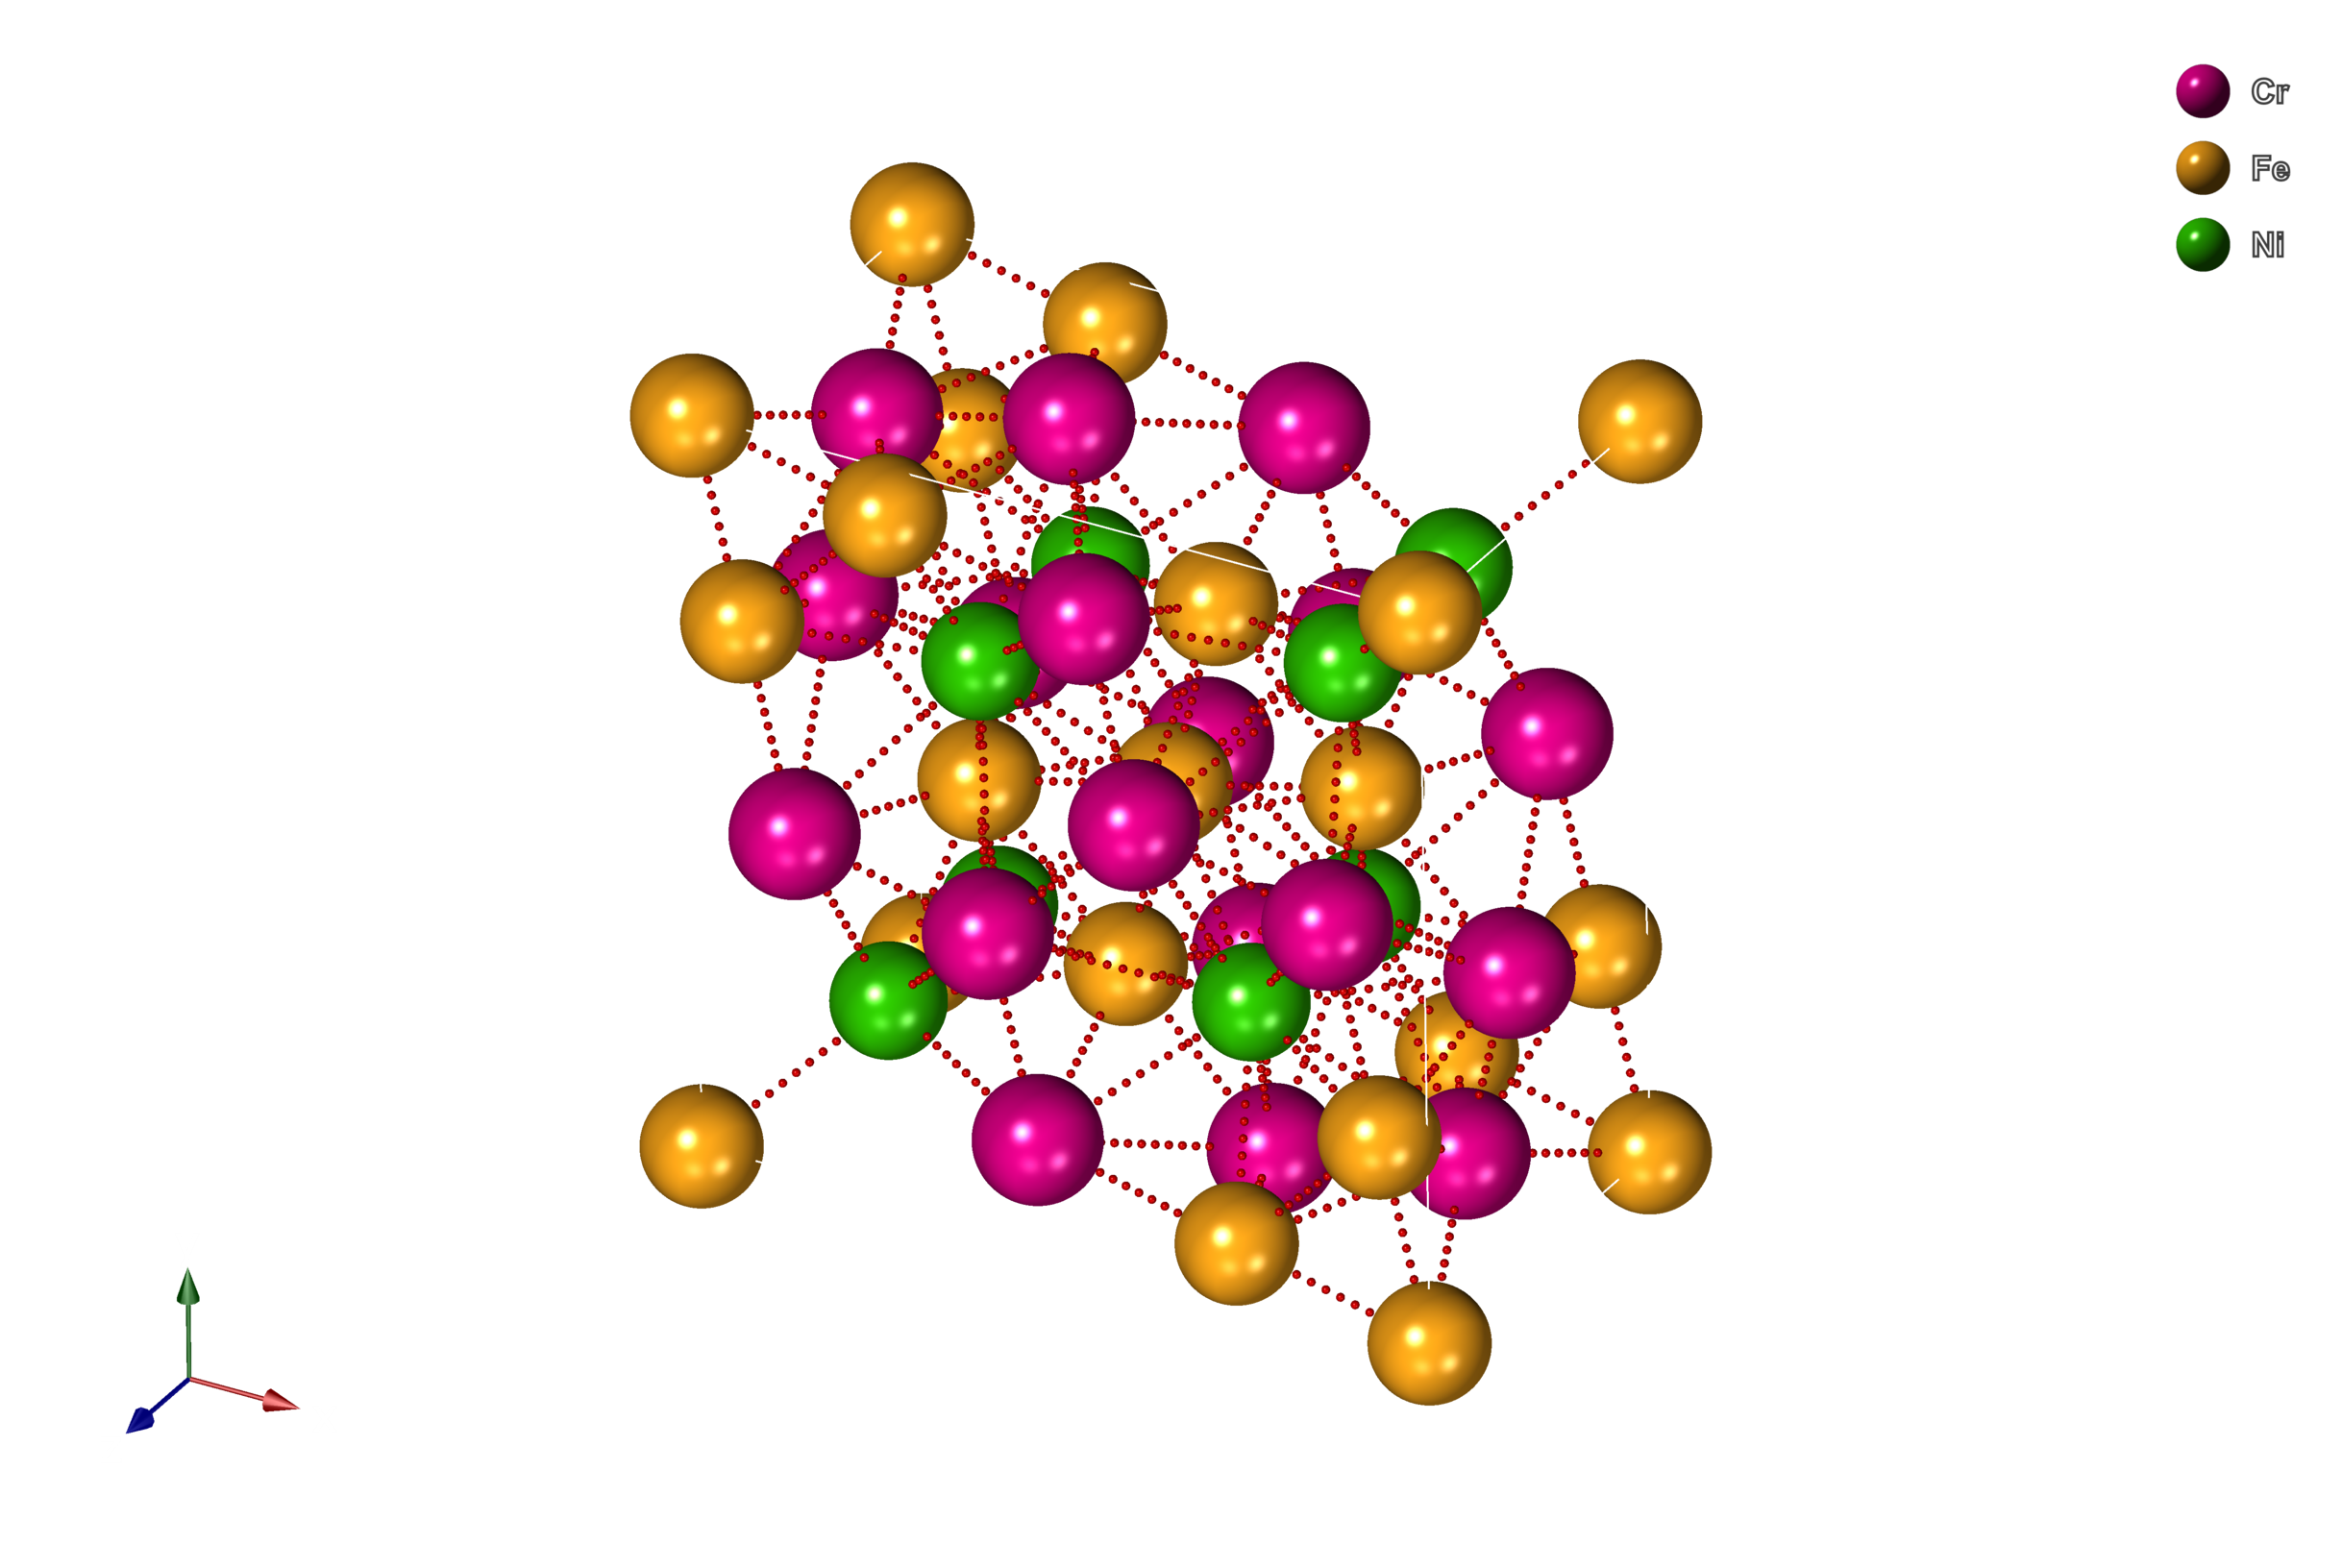
\includegraphics[width=0.6\textwidth]{pysipfennTutorial1/112-Cr12Fe10Ni8.png}
    \caption{Rendering of $Cr_{12}Fe_{10}Ni_8$ endmember occupancy of the $\sigma$-phase.}
    \label{pysipfenntutorial:simgaexample}
\end{figure}

Now, we can quickly load it into pymatgen with either (1)
\texttt{Structure.from\_file} or (2)
\texttt{pymatgen.io.vasp} module using
\texttt{Poscar} class, with the latter being more
reliable in some cases. Since it is an example of Sigma TCP phase
occupation, we will call it \texttt{baseStructure}.

\begin{minted}[xleftmargin=3\parindent, linenos=true, fontsize=\small]{python}
baseStructure = Structure.from_file("assets/0-Cr8Fe18Ni4.POSCAR")
baseStructure
\end{minted}

\begin{minted}[xleftmargin=3\parindent, fontsize=\small, bgcolor=subtlegray]{output}
Structure Summary
Lattice
    abc : 8.547048 8.547048 4.477714
 angles : 90.0 90.0 90.0
 volume : 327.10609528461225
      A : 8.547048 0.0 0.0
      B : 0.0 8.547048 0.0
      C : 0.0 0.0 4.477714
    pbc : True True True
PeriodicSite: Cr (6.305, 0.5445, 0.0) [0.7377, 0.06371, 0.0]
PeriodicSite: Cr (2.242, 8.003, 0.0) [0.2623, 0.9363, 0.0]
PeriodicSite: Cr (3.729, 2.032, 2.239) [0.4363, 0.2377, 0.5]
PeriodicSite: Cr (6.515, 4.818, 2.239) [0.7623, 0.5637, 0.5]
PeriodicSite: Cr (4.818, 6.515, 2.239) [0.5637, 0.7623, 0.5]
PeriodicSite: Cr (2.032, 3.729, 2.239) [0.2377, 0.4363, 0.5]
PeriodicSite: Cr (0.5445, 6.305, 0.0) [0.06371, 0.7377, 0.0]
PeriodicSite: Cr (8.003, 2.242, 0.0) [0.9363, 0.2623, 0.0]
PeriodicSite: Fe (0.0, 0.0, 0.0) [0.0, 0.0, 0.0]
PeriodicSite: Fe (4.274, 4.274, 2.239) [0.5, 0.5, 0.5]
PeriodicSite: Fe (3.958, 1.107, 0.0) [0.463, 0.1295, 0.0]
PeriodicSite: Fe (4.59, 7.44, 0.0) [0.537, 0.8705, 0.0]
PeriodicSite: Fe (3.167, 8.231, 2.239) [0.3705, 0.963, 0.5]
PeriodicSite: Fe (0.316, 5.38, 2.239) [0.03697, 0.6295, 0.5]
PeriodicSite: Fe (5.38, 0.316, 2.239) [0.6295, 0.03697, 0.5]
PeriodicSite: Fe (8.231, 3.167, 2.239) [0.963, 0.3705, 0.5]
PeriodicSite: Fe (1.107, 3.958, 0.0) [0.1295, 0.463, 0.0]
PeriodicSite: Fe (7.44, 4.59, 0.0) [0.8705, 0.537, 0.0]
PeriodicSite: Fe (1.562, 1.562, 1.127) [0.1827, 0.1827, 0.2517]
PeriodicSite: Fe (6.985, 6.985, 3.351) [0.8173, 0.8173, 0.7483]
PeriodicSite: Fe (6.985, 6.985, 1.127) [0.8173, 0.8173, 0.2517]
PeriodicSite: Fe (2.712, 5.835, 3.366) [0.3173, 0.6827, 0.7517]
PeriodicSite: Fe (2.712, 5.835, 1.112) [0.3173, 0.6827, 0.2483]
PeriodicSite: Fe (1.562, 1.562, 3.351) [0.1827, 0.1827, 0.7483]
PeriodicSite: Fe (5.835, 2.712, 1.112) [0.6827, 0.3173, 0.2483]
PeriodicSite: Fe (5.835, 2.712, 3.366) [0.6827, 0.3173, 0.7517]
PeriodicSite: Ni (3.418, 3.418, 0.0) [0.3999, 0.3999, 0.0]
PeriodicSite: Ni (5.129, 5.129, 0.0) [0.6001, 0.6001, 0.0]
PeriodicSite: Ni (0.8555, 7.692, 2.239) [0.1001, 0.8999, 0.5]
PeriodicSite: Ni (7.692, 0.8555, 2.239) [0.8999, 0.1001, 0.5]
\end{minted}

Now, we can quickly investigate the symmetry with tools we just learned:

\begin{minted}[xleftmargin=3\parindent, linenos=true, fontsize=\small]{python}
spgA = SpacegroupAnalyzer(baseStructure)
spgA.get_symmetrized_structure()
\end{minted}

\begin{minted}[xleftmargin=3\parindent, fontsize=\small, bgcolor=subtlegray]{output}
SymmetrizedStructure
Full Formula (Cr8 Fe18 Ni4)
Reduced Formula: Cr4Fe9Ni2
Spacegroup: P4_2/mnm (136)
abc   :   8.547048   8.547048   4.477714
angles:  90.000000  90.000000  90.000000
Sites (30)
  #  SP           a         b         c  Wyckoff
---  ----  --------  --------  --------  ---------
  0  Cr    0.737702  0.063709  0         8i
  1  Fe    0         0         0         2a
  2  Fe    0.463029  0.129472  0         8i
  3  Fe    0.182718  0.182718  0.251726  8j
  4  Ni    0.39991   0.39991   0         4f
\end{minted}

We can quickly see that our atomic configuration has \textbf{5}
chemically unique sites of different multiplicities occupied by the
\textbf{3} elements of interest. However, performing the analysis like
that can quickly lead to problems if, for instance, we introduce even a
tiny disorder in the structure, like a substitutional defect.

\begin{minted}[xleftmargin=3\parindent, linenos=true, fontsize=\small]{python}
sDilute = copy(baseStructure)
sDilute.replace(0, "Fe")
spgA = SpacegroupAnalyzer(sDilute)
spgA.get_symmetrized_structure()
\end{minted}

\begin{minted}[xleftmargin=3\parindent, fontsize=\small, bgcolor=subtlegray]{output}
SymmetrizedStructure
Full Formula (Cr7 Fe19 Ni4)
Reduced Formula: Cr7Fe19Ni4
Spacegroup: Pm (6)
abc   :   8.547048   8.547048   4.477714
angles:  90.000000  90.000000  90.000000
Sites (30)
  #  SP           a         b         c  Wyckoff
---  ----  --------  --------  --------  ---------
  0  Fe    0.737702  0.063709  0         1a
  1  Cr    0.262298  0.936291  0         1a
  2  Cr    0.436291  0.237702  0.5       1b
  3  Cr    0.762298  0.563709  0.5       1b
  4  Cr    0.563709  0.762298  0.5       1b
  5  Cr    0.237702  0.436291  0.5       1b
  6  Cr    0.063709  0.737702  0         1a
  7  Cr    0.936291  0.262298  0         1a
  8  Fe    0         0         0         1a
  9  Fe    0.5       0.5       0.5       1b
 10  Fe    0.463029  0.129472  0         1a
 11  Fe    0.536971  0.870528  0         1a
 12  Fe    0.370528  0.963029  0.5       1b
 13  Fe    0.036971  0.629472  0.5       1b
 14  Fe    0.629472  0.036971  0.5       1b
 15  Fe    0.963029  0.370528  0.5       1b
 16  Fe    0.129472  0.463029  0         1a
 17  Fe    0.870528  0.536971  0         1a
 18  Fe    0.182718  0.182718  0.251726  2c
 19  Fe    0.817282  0.817282  0.748274  2c
 20  Fe    0.317282  0.682718  0.751726  2c
 21  Fe    0.682718  0.317282  0.248274  2c
 22  Ni    0.39991   0.39991   0         1a
 23  Ni    0.60009   0.60009   0         1a
 24  Ni    0.10009   0.89991   0.5       1b
 25  Ni    0.89991   0.10009   0.5       1b
\end{minted}

Without any change to the other 29 atoms, there are 25 unique sites
rather than 5. Thus, if one wants to see what are the symmetry-enforced
unique sites, determining underlying sublattices, in the structure, one
needs anonymize the atoms first.

\begin{minted}[xleftmargin=3\parindent, linenos=true, fontsize=\small]{python}
for el in set(baseStructure.species):
    baseStructure.replace_species({el: 'dummy'})
print(baseStructure)
\end{minted}

\begin{minted}[xleftmargin=3\parindent, fontsize=\small, bgcolor=subtlegray]{output}
Full Formula (Dummy30)
Reduced Formula: Dummy
abc   :   8.547048   8.547048   4.477714
angles:  90.000000  90.000000  90.000000
pbc   :       True       True       True
Sites (30)
  #  SP              a         b         c
---  -------  --------  --------  --------
  0  Dummy0+  0.737702  0.063709  0
  1  Dummy0+  0.262298  0.936291  0
  2  Dummy0+  0.436291  0.237702  0.5
  3  Dummy0+  0.762298  0.563709  0.5
  4  Dummy0+  0.563709  0.762298  0.5
  5  Dummy0+  0.237702  0.436291  0.5
  6  Dummy0+  0.063709  0.737702  0
  7  Dummy0+  0.936291  0.262298  0
  8  Dummy0+  0         0         0
  9  Dummy0+  0.5       0.5       0.5
 10  Dummy0+  0.463029  0.129472  0
 11  Dummy0+  0.536971  0.870528  0
 12  Dummy0+  0.370528  0.963029  0.5
 13  Dummy0+  0.036971  0.629472  0.5
 14  Dummy0+  0.629472  0.036971  0.5
 15  Dummy0+  0.963029  0.370528  0.5
 16  Dummy0+  0.129472  0.463029  0
 17  Dummy0+  0.870528  0.536971  0
 18  Dummy0+  0.182718  0.182718  0.251726
 19  Dummy0+  0.817282  0.817282  0.748274
 20  Dummy0+  0.817282  0.817282  0.251726
 21  Dummy0+  0.317282  0.682718  0.751726
 22  Dummy0+  0.317282  0.682718  0.248274
 23  Dummy0+  0.182718  0.182718  0.748274
 24  Dummy0+  0.682718  0.317282  0.248274
 25  Dummy0+  0.682718  0.317282  0.751726
 26  Dummy0+  0.39991   0.39991   0
 27  Dummy0+  0.60009   0.60009   0
 28  Dummy0+  0.10009   0.89991   0.5
 29  Dummy0+  0.89991   0.10009   0.5
\end{minted}

Which we then pass to the \texttt{SpacegroupAnalyzer}
to get the symmetry information as before:

\begin{minted}[xleftmargin=3\parindent, linenos=true, fontsize=\small]{python}
spgA = SpacegroupAnalyzer(baseStructure)
spgA.get_symmetrized_structure()
\end{minted}

\begin{minted}[xleftmargin=3\parindent, fontsize=\small, bgcolor=subtlegray]{output}
SymmetrizedStructure
Full Formula (Dummy30)
Reduced Formula: Dummy
Spacegroup: P4_2/mnm (136)
abc   :   8.547048   8.547048   4.477714
angles:  90.000000  90.000000  90.000000
Sites (30)
  #  SP              a         b         c  Wyckoff
---  -------  --------  --------  --------  ---------
  0  Dummy0+  0.737702  0.063709  0         8i
  1  Dummy0+  0         0         0         2a
  2  Dummy0+  0.463029  0.129472  0         8i
  3  Dummy0+  0.182718  0.182718  0.251726  8j
  4  Dummy0+  0.39991   0.39991   0         4f
\end{minted}

Or we can turn into a useful dict for generating all possible
occupancies of the structure.

\begin{minted}[xleftmargin=3\parindent, linenos=true, fontsize=\small]{python}
spgA = SpacegroupAnalyzer(baseStructure)
uniqueDict = defaultdict(list)
for site, unique in enumerate(spgA.get_symmetry_dataset()['equivalent_atoms']):
    uniqueDict[unique] += [site]
pprint(uniqueDict)
\end{minted}

\begin{minted}[xleftmargin=3\parindent, fontsize=\small, bgcolor=subtlegray]{output}
defaultdict(<class 'list'>,
            {0: [0, 1, 2, 3, 4, 5, 6, 7],
             8: [8, 9],
             10: [10, 11, 12, 13, 14, 15, 16, 17],
             18: [18, 19, 20, 21, 22, 23, 24, 25],
             26: [26, 27, 28, 29]})
\end{minted}

\begin{minted}[xleftmargin=3\parindent, linenos=true, fontsize=\small]{python}
from itertools import product
allPermutations = list(product(['Fe', 'Cr', 'Ni'], repeat=5))
print(
    f'Obtained {len(allPermutations)} permutations of the sublattice occupancy\n'
    'E.g.:  {allPermutations[32]}')
\end{minted}

\begin{minted}[xleftmargin=3\parindent, fontsize=\small, bgcolor=subtlegray]{output}
Obtained 243 permutations of the sublattice occupancy
E.g.:  ('Fe', 'Cr', 'Fe', 'Cr', 'Ni')
\end{minted}

We can now generate them iteratively, as done below:

\begin{minted}[xleftmargin=3\parindent, linenos=true, fontsize=\small]{python}
structList = []
for permutation in allPermutations:
    tempStructure = baseStructure.copy()
    for unique, el in zip(uniqueDict, permutation):
        for site in uniqueDict[unique]:
            tempStructure.replace(site, el)
    structList.append(tempStructure)
print(structList[25])
\end{minted}

\begin{minted}[xleftmargin=3\parindent, fontsize=\small, bgcolor=subtlegray]{output}
Full Formula (Cr4 Fe10 Ni16)
Reduced Formula: Cr2Fe5Ni8
abc   :   8.547048   8.547048   4.477714
angles:  90.000000  90.000000  90.000000
pbc   :       True       True       True
Sites (30)
  #  SP           a         b         c
---  ----  --------  --------  --------
  0  Fe    0.737702  0.063709  0
  1  Fe    0.262298  0.936291  0
  2  Fe    0.436291  0.237702  0.5
  3  Fe    0.762298  0.563709  0.5
  4  Fe    0.563709  0.762298  0.5
  5  Fe    0.237702  0.436291  0.5
  6  Fe    0.063709  0.737702  0
  7  Fe    0.936291  0.262298  0
  8  Fe    0         0         0
  9  Fe    0.5       0.5       0.5
 10  Ni    0.463029  0.129472  0
 11  Ni    0.536971  0.870528  0
 12  Ni    0.370528  0.963029  0.5
 13  Ni    0.036971  0.629472  0.5
 14  Ni    0.629472  0.036971  0.5
 15  Ni    0.963029  0.370528  0.5
 16  Ni    0.129472  0.463029  0
 17  Ni    0.870528  0.536971  0
 18  Ni    0.182718  0.182718  0.251726
 19  Ni    0.817282  0.817282  0.748274
 20  Ni    0.817282  0.817282  0.251726
 21  Ni    0.317282  0.682718  0.751726
 22  Ni    0.317282  0.682718  0.248274
 23  Ni    0.182718  0.182718  0.748274
 24  Ni    0.682718  0.317282  0.248274
 25  Ni    0.682718  0.317282  0.751726
 26  Cr    0.39991   0.39991   0
 27  Cr    0.60009   0.60009   0
 28  Cr    0.10009   0.89991   0.5
 29  Cr    0.89991   0.10009   0.5
\end{minted}

\hypertarget{persisting-on-disk}{%
\subsection{Persisting on Disk}\label{pysipfenntutorial:persisting-on-disk}}

The easiest way to persist a structure on disk is to use the
\texttt{to} method of the
\texttt{Structure} object, which will write the
structure in a variety of formats, including
\texttt{POSCAR} and \texttt{CIF}:

\begin{minted}[xleftmargin=3\parindent, linenos=true, fontsize=\small]{python}
os.mkdir('POSCARs')
os.mkdir('CIFs')
for struct, permutation in zip(structList, allPermutations):
    struct.to(filename='POSCARs/' + "".join(permutation) + '.POSCAR')
    struct.to(filename='CIFs/' + "".join(permutation) + '.cif')
\end{minted}

And now we are ready to use them in a variety of other tools like DFTTK
covered last week or
\href{https://pysipfenn.readthedocs.io/en/stable/}{pySIPFENN} covered
during the next lecture!

\hypertarget{setting-up-mongodb}{%
\section{Setting up MongoDB}\label{pysipfenntutorial:setting-up-mongodb}}

With the ability to manipulate structures locally, one will quickly run
into two major problems:

\begin{itemize}
\item
  \textbf{How to pass them between personal laptop, HPC clusters, and
  lab workstations?}
\item
  \textbf{How do I share them with others later?}
\end{itemize}

One of the easiest ways to do so is to use a cloud-based database, which
will allow us to synchronize our work regardless of what machine we use
and then share it with others in a highly secure way or publicly, as
needed. In this lecture, we will use
\href{https://www.mongodb.com/atlas}{MongoDB Atlas} to set up a small
NoSQL database on the cloud. For our needs and most of the other
personal needs of researchers, the Free Tier will be more than enough,
but if you need more, you can always upgrade to a paid plan for a few
dollars a month if you need to store tens of thousands of structures.

\emph{\textbf{Note for Online Students: At this point, we will pause the
Jupiter Notebook and switch to the MongoDB Atlas website to set up the
database.} The process is fairly straightforward but feel free to stop
by during office hours for help}

Now, we should have the following: - A database called
\texttt{matse580} with a collection called
\texttt{structures} - User with read/write access named
\texttt{student} - API key for the user to access the
database (looks like \texttt{2fnc92niu2bnc9o240dc}) -
Resulting connection string to the database (looks like
\texttt{mongodb+srv://student:2fnc92niu2bnc9o240dc@<cluster\_name>/matse580})
and we can move to populating it with data!

\hypertarget{pymongo}{%
\section{Connecting Pymongo}\label{pysipfenntutorial:pymongo}}


The \texttt{pymongo} is a Python library that allows us
to interact with MongoDB databases in a very intuitive way. Let's start
by importing its \texttt{MongoClient} class and
creating a connection to our database:

\begin{minted}[xleftmargin=3\parindent, linenos=true, fontsize=\small]{python}
from pymongo import MongoClient
uri = 'mongodb+srv://amk7137:
  kASMuF5au1069Go8@cluster0.3wlhaan.mongodb.net/?retryWrites=true&w=majority'
client = MongoClient(uri)
\end{minted}

We can see what databases are available:

\begin{minted}[xleftmargin=3\parindent, linenos=true, fontsize=\small]{python}
client.list_database_names()
\end{minted}

Lets now go back to MongoDB Atlas and create a new database called
\texttt{matse580} and a collection called
\texttt{structures} in it, and hopefully see that they
are /available:

\begin{minted}[xleftmargin=3\parindent, linenos=true, fontsize=\small]{python}
client.list_database_names()
\end{minted}

\begin{minted}[xleftmargin=3\parindent, fontsize=\small, bgcolor=subtlegray]{output}
['matse580', 'admin', 'local']
\end{minted}

To go one level deeper and see what collections are available in the
\texttt{matse580} database we just created, we can use
the \texttt{list\_collection\_names} method:

\begin{minted}[xleftmargin=3\parindent, linenos=true, fontsize=\small]{python}
database = client['matse580']
database.list_collection_names()
\end{minted}

\begin{minted}[xleftmargin=3\parindent, fontsize=\small, bgcolor=subtlegray]{output}
['structures']
\end{minted}

And then read the entries in it!

\begin{minted}[xleftmargin=3\parindent, linenos=true, fontsize=\small]{python}
collection = database['structures']
\end{minted}

\begin{minted}[xleftmargin=3\parindent, linenos=true, fontsize=\small]{python}
for entry in collection.find():
    print(entry)
\end{minted}

But that's not very useful, because we didn't put anything in it yet.

\hypertarget{inserting-data}{%
\section{Inserting Data}\label{pysipfenntutorial:inserting-data}}

We start by constructing our idea of how a structure should be
represented in the database. For that purpose, we will use a dictionary
representation of the structure. This process is very flexible as NoSQL
databases like MongoDB do not require a strict schema and can be
modified on the fly and post-processed later. For our purposes, we will
use the following schema:

\begin{minted}[xleftmargin=3\parindent, linenos=true, fontsize=\small]{python}
def struct2entry(s: Structure):
    # convert to pymatgen Structure dictionary default
    strcutreDict = {'structure': s.as_dict()} 
    # convert to pymatgen Composition dictionary default
    compositionDict = {'composition': s.composition.as_dict()} 
    # merge the two dictionaries
    entry = {**strcutreDict, **compositionDict} 
    # add some extra information
    entry.update({'density': s.density,
                  'volume': s.volume,
                  'reducedFormula': s.composition.reduced_formula,
                  'weightFractions': s.composition.to_weight_dict
                  }) 
    # and a full POSCAR for easy ingestion into VASP
    entry.update({'POSCAR': s.to(fmt='poscar')})
    return entry
\end{minted}

\begin{minted}[xleftmargin=3\parindent, linenos=true, fontsize=\small]{python}
pprint(struct2entry(structList[25]))
\end{minted}

\begin{minted}[xleftmargin=3\parindent, fontsize=\small, bgcolor=subtlegray]{output}
{'POSCAR': 'Cr4 Fe10 Ni16\n'
           ...,
 'composition': {'Cr': 4.0, 'Fe': 10.0, 'Ni': 16.0},
 'density': 8.658038607159655,
 'reducedFormula': 'Cr2Fe5Ni8',
 'structure': {'@class': 'Structure',
               '@module': 'pymatgen.core.structure',
               'charge': 0,
               'lattice': {'a': 8.547048,
                           'alpha': 90.0,
                           'b': 8.547048,
                           'beta': 90.0,
                           'c': 4.477714,
                           'gamma': 90.0,
                           'matrix': [[8.547048, 0.0, 0.0],
                                      [0.0, 8.547048, 0.0],
                                      [0.0, 0.0, 4.477714]],
                           'pbc': (True, True, True),
                           'volume': 327.10609528461225},
               'properties': {},
               'sites': [{'abc': [0.737702, 0.063709, 0.0],
                          'label': 'Fe',
                          'properties': {},
                          'species': [{'element': 'Fe', 'occu': 1}],
                          'xyz': [6.305174403696, 0.544523881032, 0.0]},
                         ...
                         ]},
 'volume': 327.10609528461225,
 'weightFractions': {'Cr': 0.12194716383563854,
                     'Fe': 0.3274351039982438,
                     'Ni': 0.5506177321661175}}
\end{minted}

Looks great! Now we can add some metadata to it, like who created it,
when, and what was the permutation label used to generate it earlier; to
then insert it into the database using the
\texttt{insert\_one} method, which is not the fastest,
but the most flexible way to do so:

\begin{minted}[xleftmargin=3\parindent, linenos=true, fontsize=\small]{python}
for struct, permutation in zip(structList, allPermutations):
    entry = struct2entry(struct)
    entry.update({'permutation': "".join(permutation),
                  'autor': 'Happy Student',
                  'creationDate': datetime.now(ZoneInfo('America/New_York'))
                })
    collection.insert_one(entry)
\end{minted}

We can now quickly check if they are present by counting the number of
entries in the collection:

\begin{minted}[xleftmargin=3\parindent, linenos=true, fontsize=\small]{python}
collection.count_documents({})
\end{minted}

\begin{minted}[xleftmargin=3\parindent, fontsize=\small, bgcolor=subtlegray]{output}
243
\end{minted}

If something went wrong halfway, you can start over by deleting all
entries in the collection (be careful with this one!):

\begin{minted}[xleftmargin=3\parindent, linenos=true, fontsize=\small]{python}
# Uncomment to run
#collection.delete_many({})
#collection.count_documents({})
\end{minted}

\hypertarget{updating-data}{%
\subsection{Updating Data}\label{pysipfenntutorial:updating-data}}

This will be reiterated in the next lecture, but in principle updating
the data is easy. For example, we can add a new field to the document,
like \texttt{averageElectronegativity} by iterating
over all entries present in the collection and calculating it:

\begin{minted}[xleftmargin=3\parindent, linenos=true, fontsize=\small]{python}
for entry in collection.find():
    id = entry['_id']
    s = Structure.from_dict(entry['structure'])
    collection.update_one(
        {'_id': id}, 
        {'$set': {'averageElectronegativity': s.composition.average_electroneg}})
\end{minted}

Or, to remove a field, like \texttt{volume}, which
happens to be the same for all structures, we can do it in a similar
way:

\begin{minted}[xleftmargin=3\parindent, linenos=true, fontsize=\small]{python}
for entry in collection.find():
    id = entry['_id']
    collection.update_one({'_id': id}, {'$unset': {'volume': ''}})
\end{minted}

Since we apply it in the same way on all entries, we can do it in a
single line of code using the \texttt{update\_many}
method and an empty filter \texttt{\{\}} querying all
entries:

\begin{minted}[xleftmargin=3\parindent, linenos=true, fontsize=\small]{python}
collection.update_many({}, {'$unset': {'volume': ''}})
\end{minted}

\begin{minted}[xleftmargin=3\parindent, fontsize=\small, bgcolor=subtlegray]{output}
<pymongo.results.UpdateResult at 0x294323340>
\end{minted}

\hypertarget{querying-data}{%
\subsection{Querying Data}\label{pysipfenntutorial:querying-data}}

Now that we have some data in the database, we can start querying it.
MongoDB has state-of-the-art query language that allows us to do very
complex queries and do them with extreme performance. You can find more
information about it
\href{https://www.mongodb.com/docs/manual/reference/method/db.collection.find/\#db.collection.find}{in
this documentation} but for our purposes, we will stick to the basics
like finding all Cr-containing structures.

To find all entries in the collection, we can use the
\texttt{find} method with a dictionary of query
parameters. We can use many different methods, but the simplest would be
to look for a composition dictionary with over-0 or non-empty values for
Cr:

\begin{minted}[xleftmargin=3\parindent, linenos=true, fontsize=\small]{python}
for entry in collection.find({'weightFractions.Cr': {'$gt': 0}}):
    print(entry['reducedFormula'])
\end{minted}

\begin{minted}[xleftmargin=3\parindent, fontsize=\small, bgcolor=subtlegray]{output}
Cr2Fe13
Cr4Fe11
Cr2Fe3
Cr4Fe9Ni2
Cr2Fe9Ni4
Cr4Fe11
...
\end{minted}

\begin{minted}[xleftmargin=3\parindent, linenos=true, fontsize=\small]{python}
for entry in collection.find({'weightFractions.Cr': {'$ne': None}}):
    print(entry['reducedFormula'])
\end{minted}

\begin{minted}[xleftmargin=3\parindent, fontsize=\small, bgcolor=subtlegray]{output}
Cr2Fe13
Cr4Fe11
Cr2Fe3
Cr4Fe9Ni2
Cr2Fe9Ni4
Cr4Fe11
...
\end{minted}

Or to get a specific permutation, we can use
\texttt{find\_one} method, which will return the first
entry matching the query:

\begin{minted}[xleftmargin=3\parindent, linenos=true, fontsize=\small]{python}
originalStruct25 = collection.find_one({'permutation': 'FeFeNiNiCr'})
originalStruct25['reducedFormula']
\end{minted}

\begin{minted}[xleftmargin=3\parindent, fontsize=\small, bgcolor=subtlegray]{output}
'Cr2Fe5Ni8'
\end{minted}

\hypertarget{pysipfenn-install}{%
\section{pySIPFENN Install}\label{pysipfenntutorial:pysipfenn-install}}

The last quick thing we will do today is to install pySIPFENN, which is
a Python framework which, among other things, allows us to quickly
predict stability of materials using machine learning. It can be
installed using \texttt{pip} just like pymatgen:

\begin{minted}[xleftmargin=3\parindent, linenos=true, fontsize=\small]{python}
#!pip install pysipfenn
\end{minted}

The reason we are installing it here is that the employed models are
fairly large and may take a while to download, unless you use cloud
virtual machine like GitHub Codespaces. Thus, we will start it now so
that it is ready for next week's lecture. Process is automated and you
just need to initialize an empty \texttt{Calculator}
object:

\begin{minted}[xleftmargin=3\parindent, linenos=true, fontsize=\small]{python}
from pysipfenn import Calculator
c = Calculator()
\end{minted}

\begin{minted}[xleftmargin=3\parindent, fontsize=\small, bgcolor=subtlegray, breaklines]{output}
*********  Initializing pySIPFENN Calculator  **********
Loading model definitions from: ...
Found 4 network definitions in models.json
  SIPFENN_Krajewski2020 Standard Materials Model
  SIPFENN_Krajewski2020 Novel Materials Model
  SIPFENN_Krajewski2020 Light Model
  SIPFENN_Krajewski2022 KS2022 Novel Materials Model
Loading all available models (autoLoad=True)
Loading models:

100%|||||||||||||||||||||||||||||||| 4/4 [00:14<00:00,  3.63s/it]

*********  pySIPFENN Successfully Initialized  **********
\end{minted}

And then, order it to download the models:

\begin{minted}[xleftmargin=3\parindent, linenos=true, fontsize=\small]{python}
c.downloadModels()
\end{minted}

\begin{minted}[xleftmargin=3\parindent, fontsize=\small, bgcolor=subtlegray]{output}
Fetching all networks!
All networks available!
  SIPFENN_Krajewski2020 Standard Materials Model
  SIPFENN_Krajewski2020 Novel Materials Model
  SIPFENN_Krajewski2020 Light Model
  SIPFENN_Krajewski2022 KS2022 Novel Materials Model
\end{minted}

It should take 1-30 minutes depending on your internet connection, but
once it is done they will be available until the package is uninstalled.
Also, you can run this command as many times as you want, and it will
only download the models that are not yet present on your system.
